\documentclass[a4paper, 12pt]{report}

%%%%%%%%%%%%
% Packages %
%%%%%%%%%%%%

\usepackage[english]{babel}
\usepackage[noheader]{packages/sleek}
\usepackage{packages/sleek-title}
\usepackage{packages/sleek-theorems}
\usepackage{packages/sleek-listings}
\usepackage{hyperref}

%%%%%%%%%%%%%%
% Title-page %
%%%%%%%%%%%%%%

\logo{./resources/pdf/logo.pdf}
\institute{Universitas Semarang}
\faculty{Fakultas Teknologi Informasi dan Komunikasi}
\department{Teknik Informatika}
\title{TIS18430P\\Open Source Systems}
\subtitle{Modul Praktikum Mahasiswa}
\author{\textit{Oleh:}\\Alauddin Maulana Hirzan, S. Kom., M. Kom\\0607069401}
\date{}

\lstdefinestyle{latex}{
    language=TeX,
    style=default,
    commentstyle=\ForestGreen,
    keywordstyle=\TrueBlue,
    stringstyle=\VeronicaPurple,
    emphstyle=\TrueBlue,
    emph={LaTeX, usepackage, textit, textbf, textsc}
}

\FrameTBStyle{latex}

%%%%%%%%%%%%%%
% Rename %
%%%%%%%%%%%%%%

\def\tbs{\textbackslash}
\addto\captionsenglish{\renewcommand{\chaptername}{Bab}}
\addto\captionsenglish{\renewcommand{\contentsname}{Daftar Isi}}
\addto\captionsenglish{\renewcommand{\figurename}{Gambar}}
\addto\captionsenglish{\renewcommand{\tablename}{Tabel}}
\addto\captionsenglish{\renewcommand{\listfigurename}{Daftar Gambar}}
\addto\captionsenglish{\renewcommand{\listtablename}{Daftar Tabel}}

%%%%%%%%%%%%%%
% Usable Commands %
%%%%%%%%%%%%%%

% Chapter
% \chapter{}

% Section
% \section{}
% \subsection{}

% Footnotes
% \blindfootnote

% Listing
% \begin{lstlisting}[style=latexFrameTB, caption={Example of Sleek Template packages usage.}, gobble=8]
%	\usepackage[english]{babel}
%	\usepackage[noheader]{packages/sleek}
%	\usepackage{packages/sleek-title}
% \end{lstlisting}

% Numbering
%\begin{enumerate}[noitemsep]
%	\item \texttt{parindent} add indentation to the first line of paragraphs;
%	\item \texttt{noheader} removes the document header;
%	\item \texttt{french} changes the decimal sign to a comma and translates some captions.
%\end{enumerate}

% Figure
%\begin{figure}[H]
%	\centering
%	
\includegraphics[width=0.5\textwidth]{resources/pdf/logo.pdf}
%	\noskipcaption{}
%	\label{}
%\end{figure}

% Table
%\begin{table}[H]
%	\centering
%	\begin{tabular}{|r|r|c|l|}
%		\hline
%		\multicolumn{3}{|l|}{a} & qrs  \\ \hline
%		b &  ef &     jkl      & tuvx \\ \hline
%		cd & ghi &     mnop     & wyz  \\ \hline
%	\end{tabular}
%	\caption{Example of multi-column cells.}
%	\label{tab:multicol_example}
%\end{table}

%%%%%%%%%%%%
% Document %
%%%%%%%%%%%%

\begin{document}
    \maketitle
    \romantableofcontents
    \listoffigures

	%%%%%%%%%%%%%%
	% Bab 1 %
	%%%%%%%%%%%%%%

    \chapter{Pendahuluan}
	\section {Mengenal \textit{Version Control System} dan GIT}
    \textbf{\textit{Version Control}} di dalam bidang \textit{Software Engineering} merupakan sebuah teknik yang dilakukan untuk mengendalikan versi yang akan dirilis dalam pengembangan aplikasi. Sehingga dengan adanya teknik ini, semua perubahan yang terjadi di dalam aplikasi tersebut dapat tercatat dan termonitor dengan baik. Terdapat beberapa \textit{software} yang dapat digunakan seperti GIT dan SVN. Keduanya memiliki tugas yang sama namun cara mencapai tugas itu berbeda. Dalam praktikum kali ini, mata kuliah ini menganjurkan untuk menggunakan GIT sebagai alat pengendalian versi.
  	
  	Apa itu GIT? GIT adalah aplikasi pengendali versi yang menyimpan dan menganalisis informasi dengan cara yang berbeda dengan yang lainnya. GIT menerapkan konsep \textit{content-aware} sehingga dia tidak akan menambahkan, mengubah, mengunggah file yang kosong atau tidak mengalami perubahan. Ciri khas ini dimiliki oleh GIT namun tidak dimiliki oleh aplikasi lain. Aplikasi lain seperti CSV, Subversion, Perforce, Bazaar menggunakan pendakatan \textit{time-based changes} atau melihat perubahan file dari waktu ke waktu. Atau bisa dikenal sebagai \textit{delta-based version control}. Berikut ini adalah perbandingan antara \textit{Delta-based} dengan \textit{Snapshot-based} GIT:
  	
  	\begin{figure}[H]
  		\centering
  		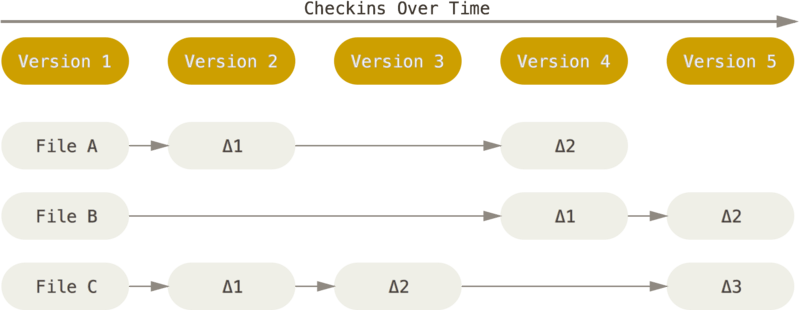
\includegraphics[width=1.0\textwidth]{figures/delta.png}
  		\noskipcaption{\textit{Delta-based Control}}
  		\label{fig.delta}
  	\end{figure}
  
  Model yang ditunjukkan oleh Gambar \ref{fig.delta} adalah cara yang digunakan oleh aplikasi lainnya. Dengan membandingkan perbedaan antara satu file dengan yang lainnya (\textit{diff} atau \textit{delta}), VCS akan mengubah file tersebut. Jika di file A terdapat perubahan kedua, maka perubahan tersebut akan diunggah. Jika tidak, maka file akan dibiarkan.
  
  \begin{figure}[H]
  	\centering
  	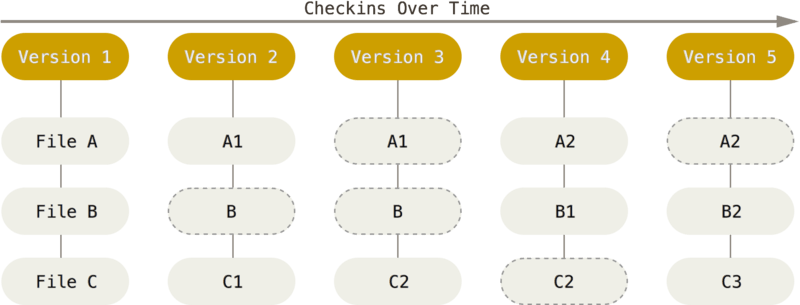
\includegraphics[width=1.0\textwidth]{figures/snapshots.png}
  	\noskipcaption{\textit{Snapshot-based Control}}
  	\label{fig.snapshot}
  \end{figure}

	Sedangkan GIT yang menggunakan metode \textbf{\textit{snapshot}}, menggunakan cara yang berbeda dalam mengendalikan versi dari masing-masing file. Dengan menggunakan GIT setiap perintah \textbf{\textit{commit}} yang diberikan, GIT akan merekam status file yang ada di folder tersebut dan menungunggahnya. Sehingga disetiap sesi \textbf{\textit{commit}} versi, file-file yang dibutuhkan tetap ada. Sehingga muncul fitur seperti \textbf{\textit{branching}} yang memungkinkan perubahan tanpa menyentuh file utama.
	
	\section{Keamanan dan Integritas GIT}
	
	GIT memiliki perlindungan serta integritas yang sangat tinggi. Pengguna dapat mengunggah file mereka melalui jalur yang aman melalui \textbf{\textit{Secure Shell / SSH}}. Selain itu, GIT juga melakukan monitoring kualitas atau perubahan file berdasarkan \textbf{\textit{checksum hash}} menggunakan SHA-1. Ditambah, untuk memastikan orang-orang yang mengunggah adalah orang asli bukan penuri, GIT juga mampu menggunakan kunci kriptografi sebagai identifikasi \textbf{\textit{commiter}}.
	
	\section{Cara Kerja GIT}
  	
  	GIT memiliki cara kerja yang sangat sederhana, hanya menggunakan \textbf{Tiga Tahapan} saja. Berikut adalah ilustrasi cara kerja GIT:
  	
  	\begin{figure}[H]
  		\centering
  		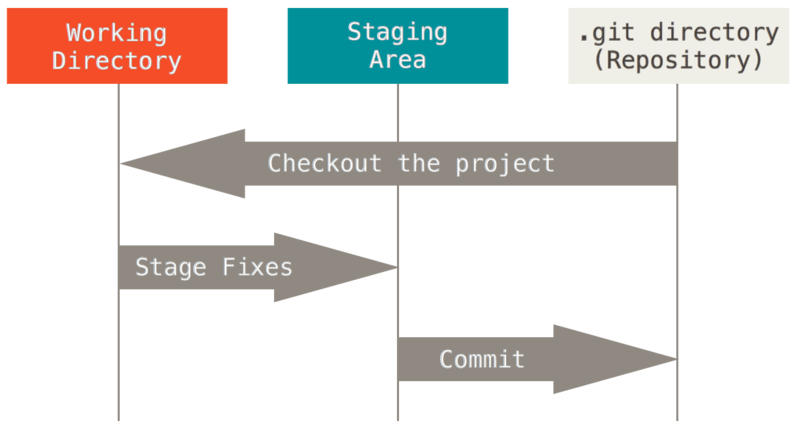
\includegraphics[width=1.0\textwidth]{figures/areas.png}
  		\noskipcaption{Tiga Tahapan GIT}
  		\label{fig.tahapan}
  	\end{figure}
  
  Menurut Gambar \ref{fig.tahapan}, GIT dimulai dengan melakukan \textbf{\textit{checkout}} pada projek yang ada di dalam folder. Hal ini bisa dicapat dengan melakukan perintah \textbf{\textit{git init}} untuk memulai GIT, atau dengan mengambil projek yang sudah ada melalui perintah \textbf{\textit{git clone}}. Folder \textbf{.git} ini berisi informasi-informasi penting berkaitan dengan projek tersebut. Meski aman untuk dihapus, namun rekam jejak file termasuk link upload akan hilang.
  
  Setelah melakukan inisialisasi atau klon, pengguna dapat melakukan perubahan file tersebut. Segala bentuk perubahan inilah yang nantinya akan masuk ke dalam \textbf{\textit{Staging Area}} melalui perintah \textbf{\textit{git add -A}}. Semua file yang masuk di tahap ini kemudian diberi label menggunakan perintah \textbf{\textit{git commit}} sehingga memudahkan pengguna dalam membaca versi yang diunggah. \textbf{\textit{Commit}} ini disimpan dalam folder \textbf{.git}. File-file siap diunggah ke \textbf{\textit{Repository}}
  
  \section{Respository Penyimpanan}
  	
  \textbf{\textit{Repository}} merupakan tempat penyimpanan kode-kode atau gambar atau file lain (dengan batas ukuran tertentu) secara daring sehingga bisa diakses oleh orang lain. Hampir mirip dengan \textit{Cloud Storage} pada biasanya, tetapi hanya bisa diakses oleh pemilik atau \textbf{\textit{contributor}} yang sudah dipercaya (dan diberi akses). Di dunia internet ada beberapa repositori yang bisa dipakai seperti \url{https://github.com} atau \url{https://gitlab.com}. Keduanya memiliki tugas yang sama sebagai repositori, namun memiliki kebijakan yang berbeda dalam hal prinsip \textit{open source}. Dalam hal fitur, \textit{GitHub} lebih banyak kebebasan dibandingkan \textit{GitLab}.
  
  %%%%%%%%%%%%%%
  % Bab 2 %
  %%%%%%%%%%%%%%
  
  \chapter{Persiapan Praktikum}
  
  Agar praktikum dapat berjalan dengan lancar, mahasiswa diwajibkan memenuhi persyaratan berikut baik dalam bentuk perangkat keras maupun lunak:
  
  \section{Perangkat Keras}
  
  GIT SCM tidak memerlukan spesifikasi yang tinggi untuk dioperasikan sehingga dapat digunakan diperangkat sekelas \textit{Raspberry Pi} dengan spesifikasi paling rendah. Namun wajib memiliki
  
  \begin{itemize}
  	\item Layar Monitor
  	\item Mouse
  	\item Keyboard
  \end{itemize}

\section{Perangkat Lunak}

Perangkat lunak berikut ini wajib diinstall oleh mahasiswa demi lancarnya praktikum:
\begin{itemize}
	\item Pengguna Windows
	\begin{enumerate}
		\item Git-SCM via \url{https://git-scm.com/} (Gratis)
		\item GPG4Win via \url{https://gpg4win.org/download.html} (Gratis, pilih \$0 ketika mengunduh)
		\item Notepad (sudah termasuk)
	\end{enumerate}
	\item Pengguna Linux
	\begin{enumerate}
		\item git
		\item gpg
		\item nano atau vim atau editor lain
	\end{enumerate}
\end{itemize}

\section{Instalasi}

	Dalam melakukan instalasi GIT, ada satu langkah yang harus diperhatikan. Langkah ini akan menentukan editor apa yang akan dipakai git di Windows.
	
	\begin{figure}[H]
		\centering
		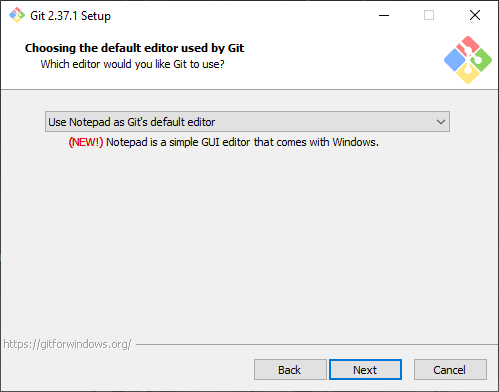
\includegraphics[width=0.8\textwidth]{figures/installer.png}
		\noskipcaption{Tahap Pemilihan Editor}
		\label{fig.installer}
	\end{figure}

	Pastikan ketika memasang GIT-SCM untuk memilih \textbf{\textit{Notepad}} sebagai editor default Windows. Bagian akhir ketika praktikum, mahasiswa sebaiknya menggunakan \textbf{\textit{Git Bash}} dan bukan menggunakan CMD maupun Powershell seperti Gambar \ref{fig.gitbash}. 
	
	\begin{figure}[H]
		\centering
		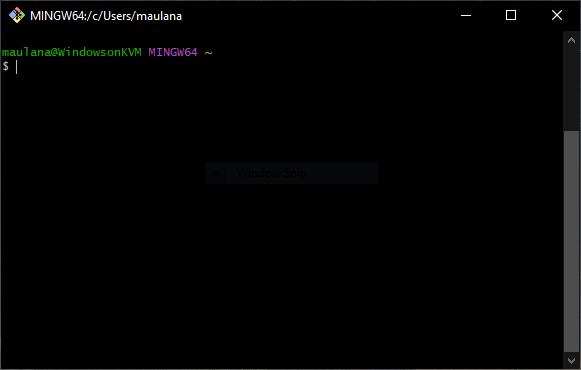
\includegraphics[width=0.8\textwidth]{figures/git-bash.png}
		\noskipcaption{Git Bash}
		\label{fig.gitbash}
	\end{figure}

	\section{Akun GitHub}
	\subsection{Daftar Akun}
	Tahapan ini sangat penting karena git tidak bisa beroperasi tanpa akun di \textit{GitHub}. Buka website \url{https://github.com/signup}. Isi semua form yang diperlukan, dan pastikan untuk \textbf{konfirmasi e-mail} agar akun GitHub dapat digunakan.
	
	\begin{figure}[H]
		\centering
		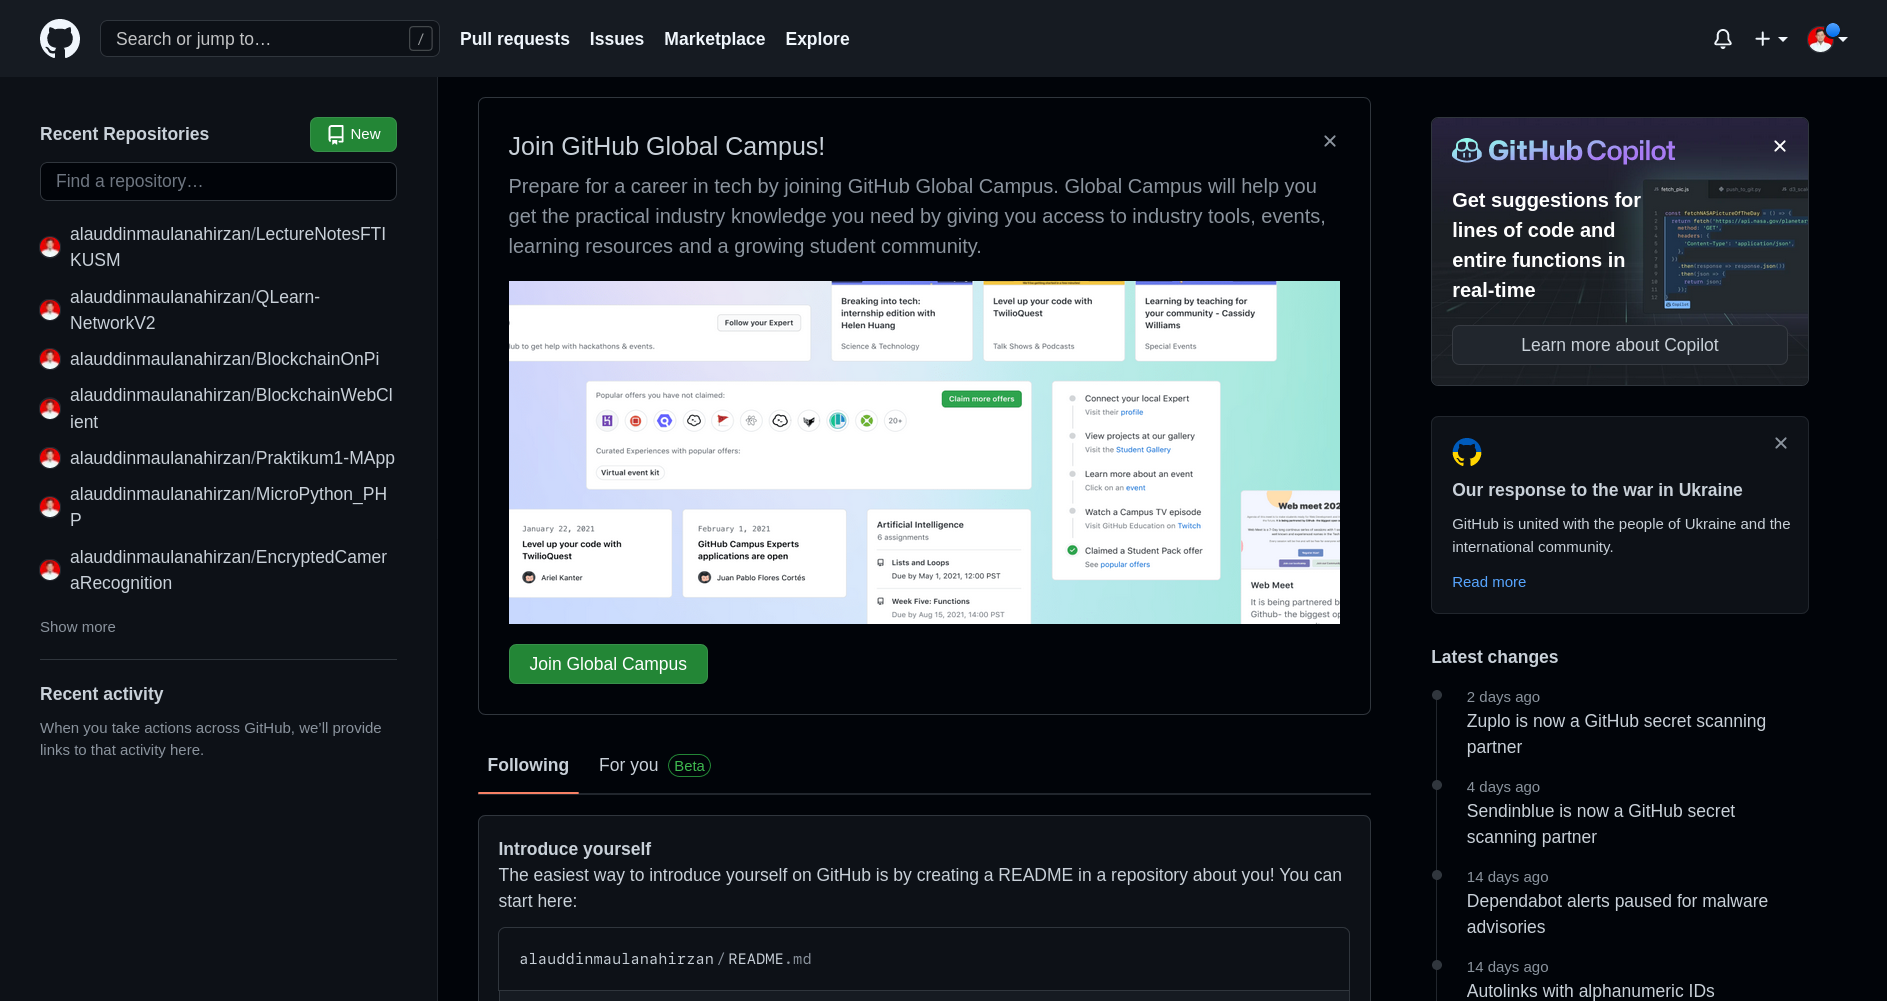
\includegraphics[width=1.0\textwidth]{figures/github.com.png}
		\noskipcaption{Git Bash}
		\label{fig.githubcom}
	\end{figure}

	\subsection{\textit{Personal Token Access}}
	Tahapn ini sangat penting karena demi keamanan pemilik GitHub untuk menggunakan \textit{Token} ketika mengunggah kodenya. Cukup dengan cara mudah:
	
	\begin{enumerate}
		\item Klik \textbf{Foto Profil} di \textbf{Pojok Kanan Atas}, Pilih \textbf{Settings}
		\begin{figure}[H]
			\centering
			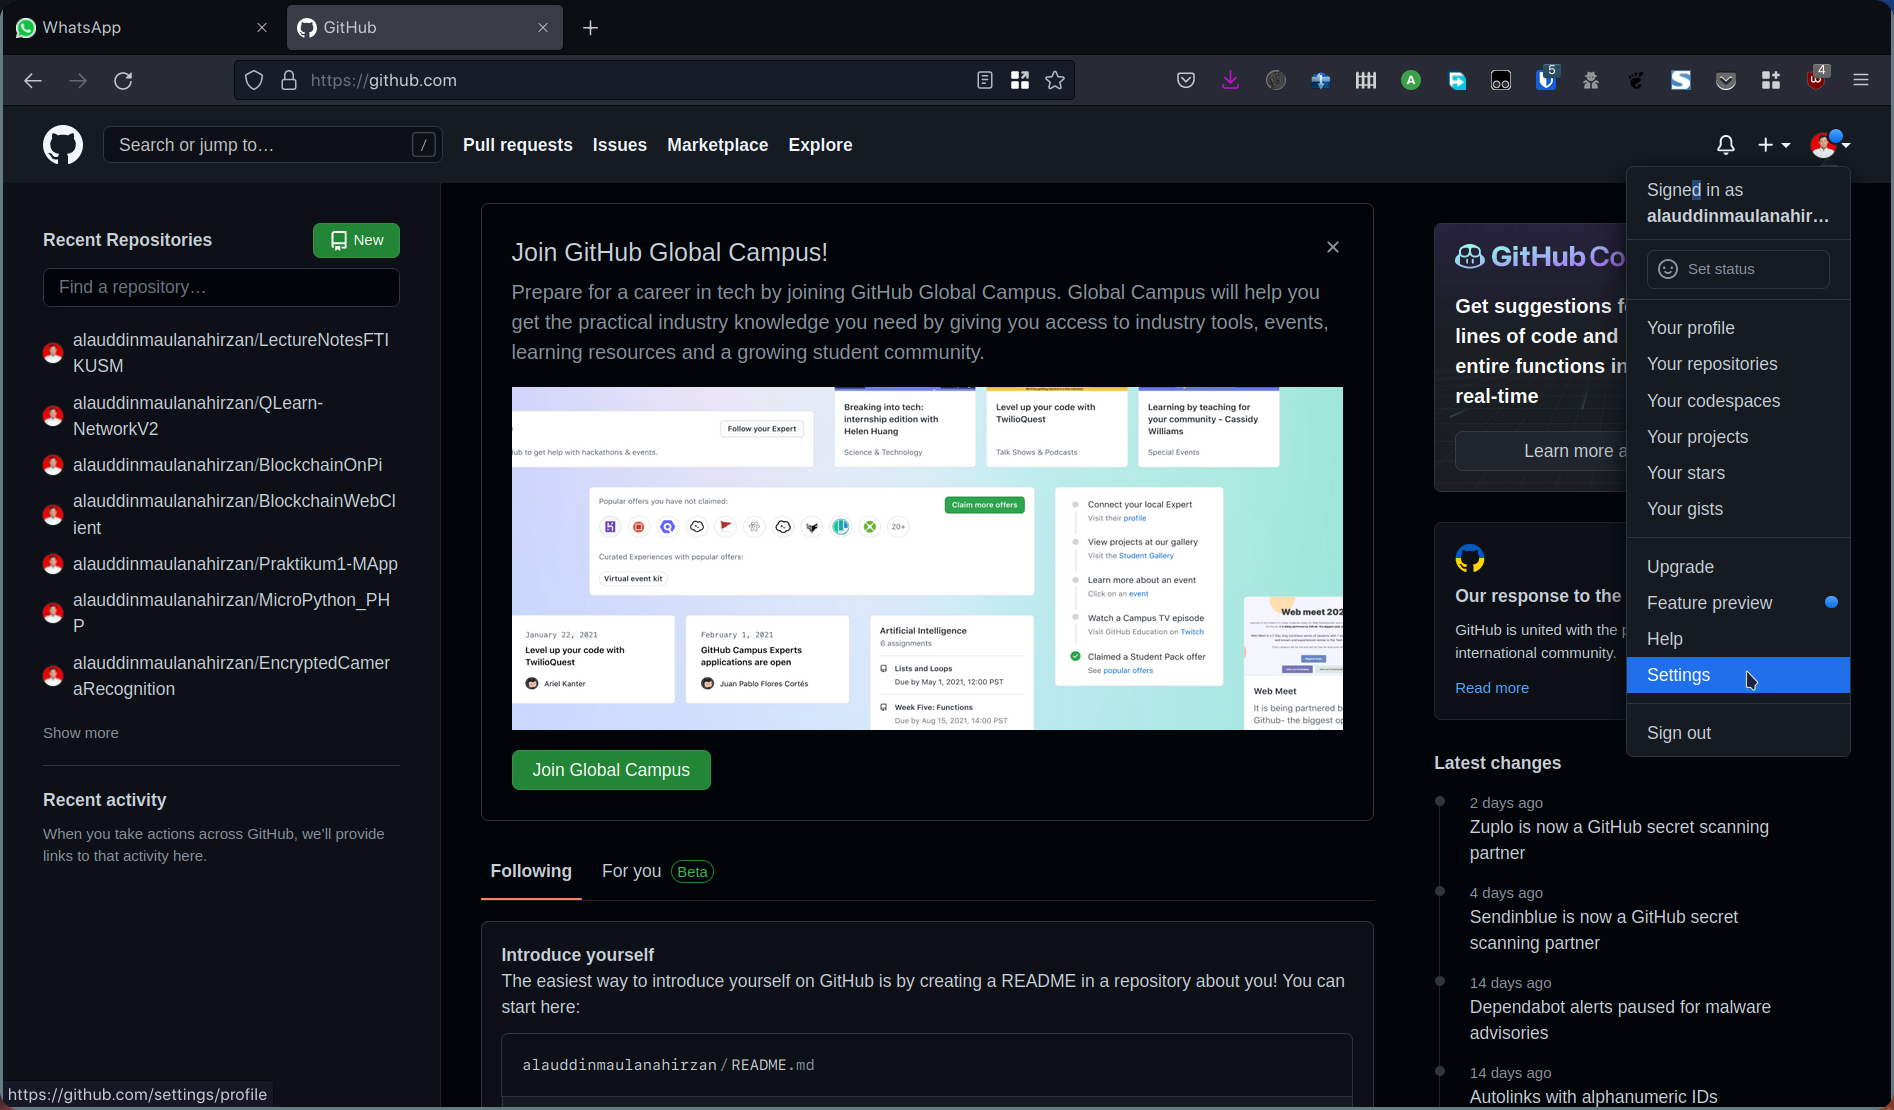
\includegraphics[width=0.8\textwidth]{figures/token1.png}
			\label{fig.token1}
		\end{figure}
		\item Klik \textbf{Developer Settings} di bagian bawah kiri
		\begin{figure}[H]
			\centering
			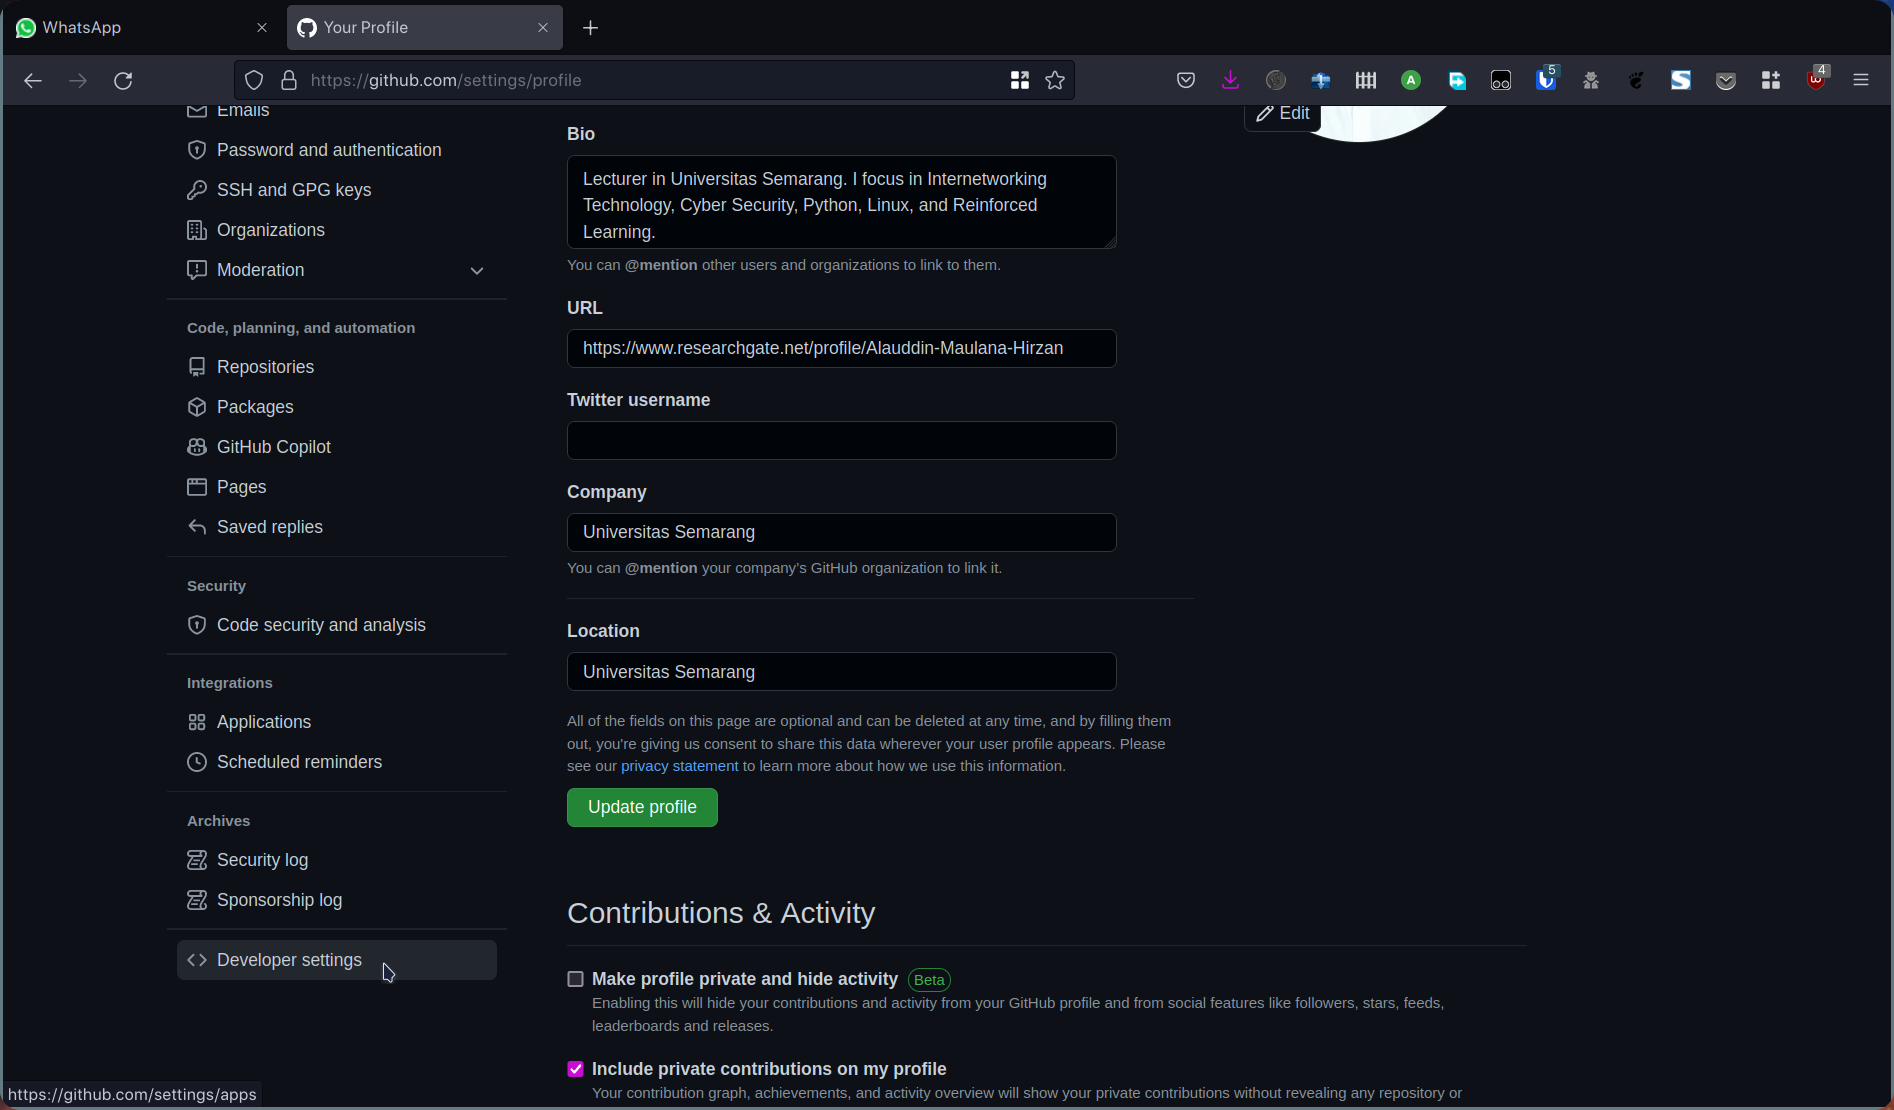
\includegraphics[width=0.8\textwidth]{figures/token2.png}
			\label{fig.token2}
		\end{figure}
		\item Pilih \textbf{Personal access token}, lalu klik \textbf{Generate new token}
		\begin{figure}[H]
			\centering
			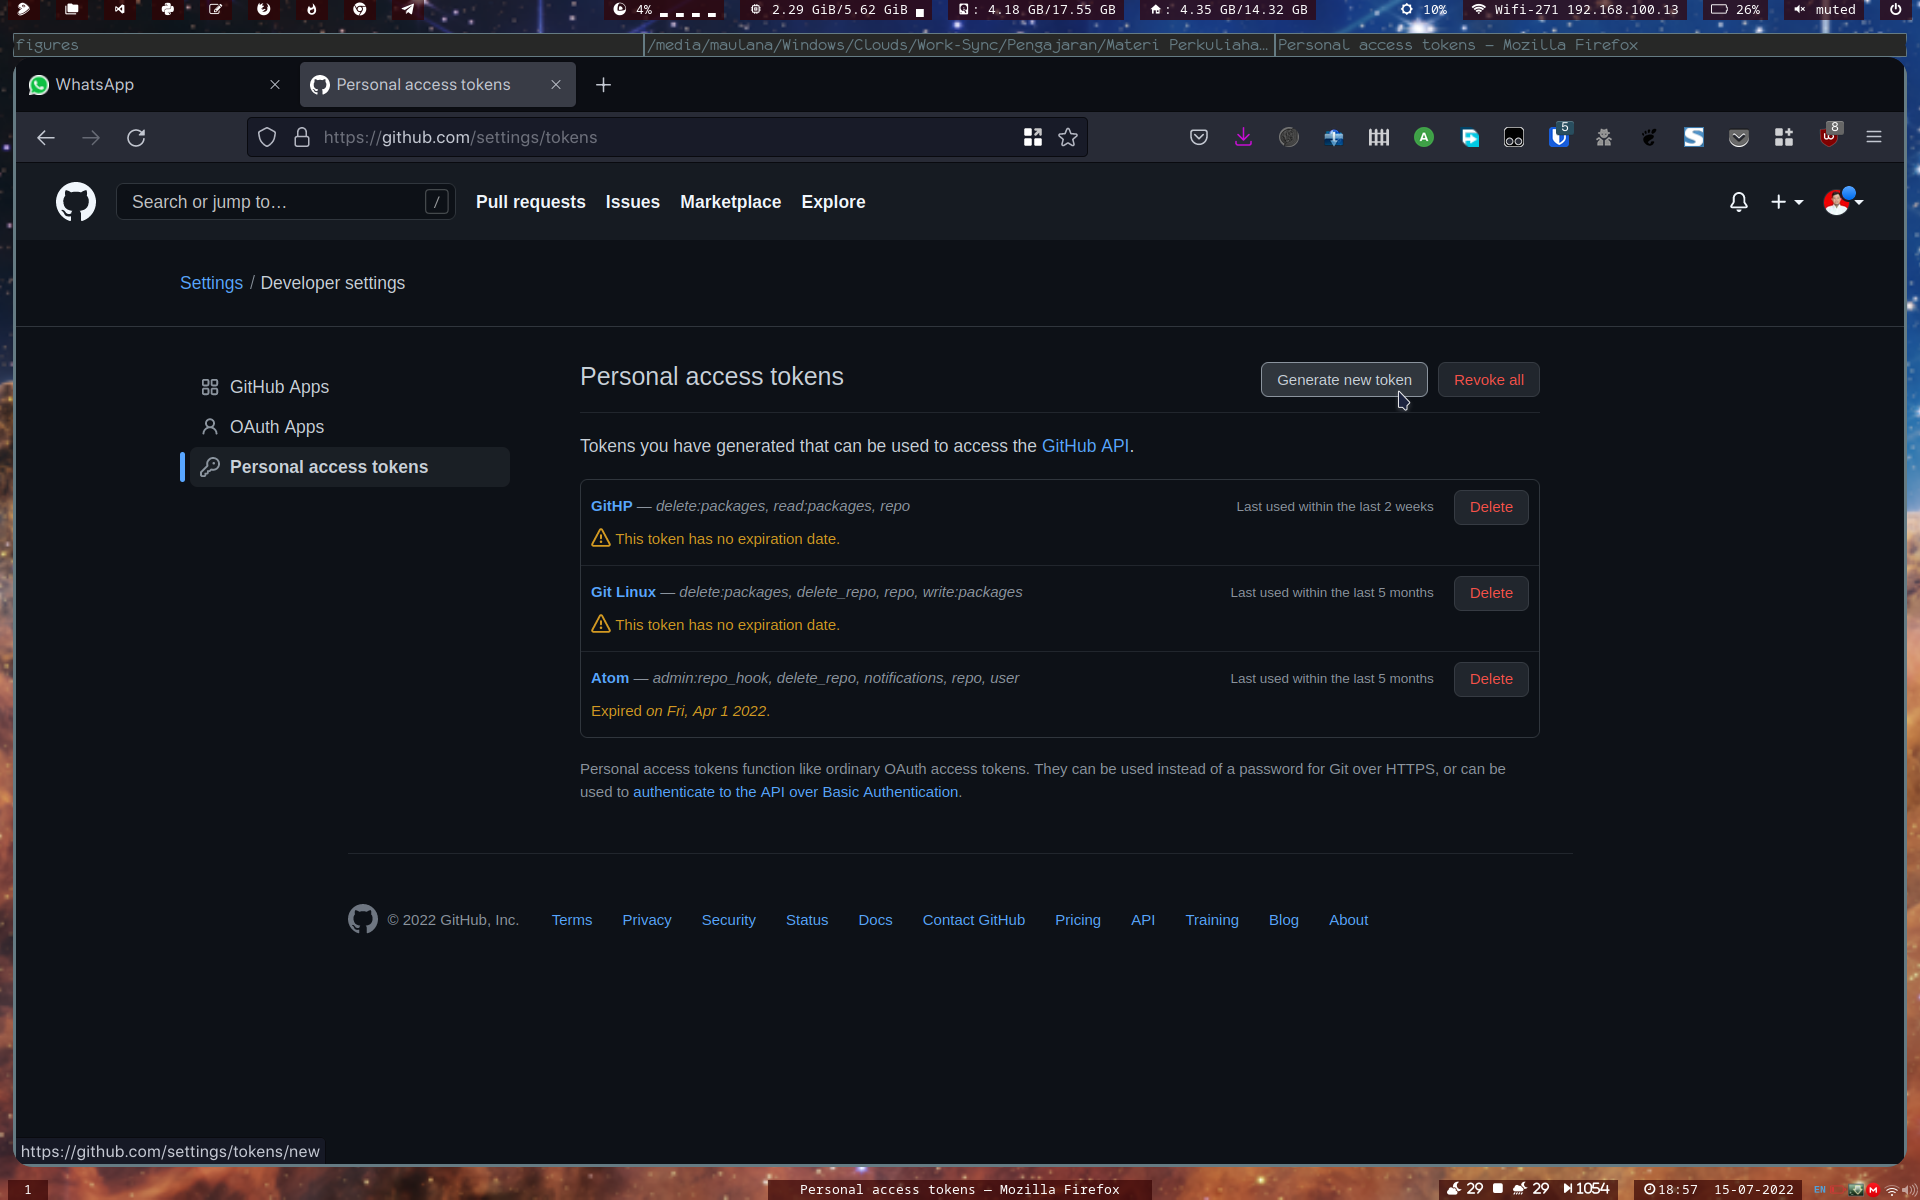
\includegraphics[width=0.8\textwidth]{figures/token3.png}
			\label{fig.token3}
		\end{figure}
		\item \textbf{GitHub} akan meminta \textbf{Password}. Masukkan \textbf{Password} akun.
		\item \textbf{Beri} nama token. Ubah \textbf{Expiration} ke \textbf{No expiration} dan centang \textbf{semua scope}. Jika sudah klik \textbf{Generate token} yang ada di bawah halaman.
		\begin{figure}[H]
			\centering
			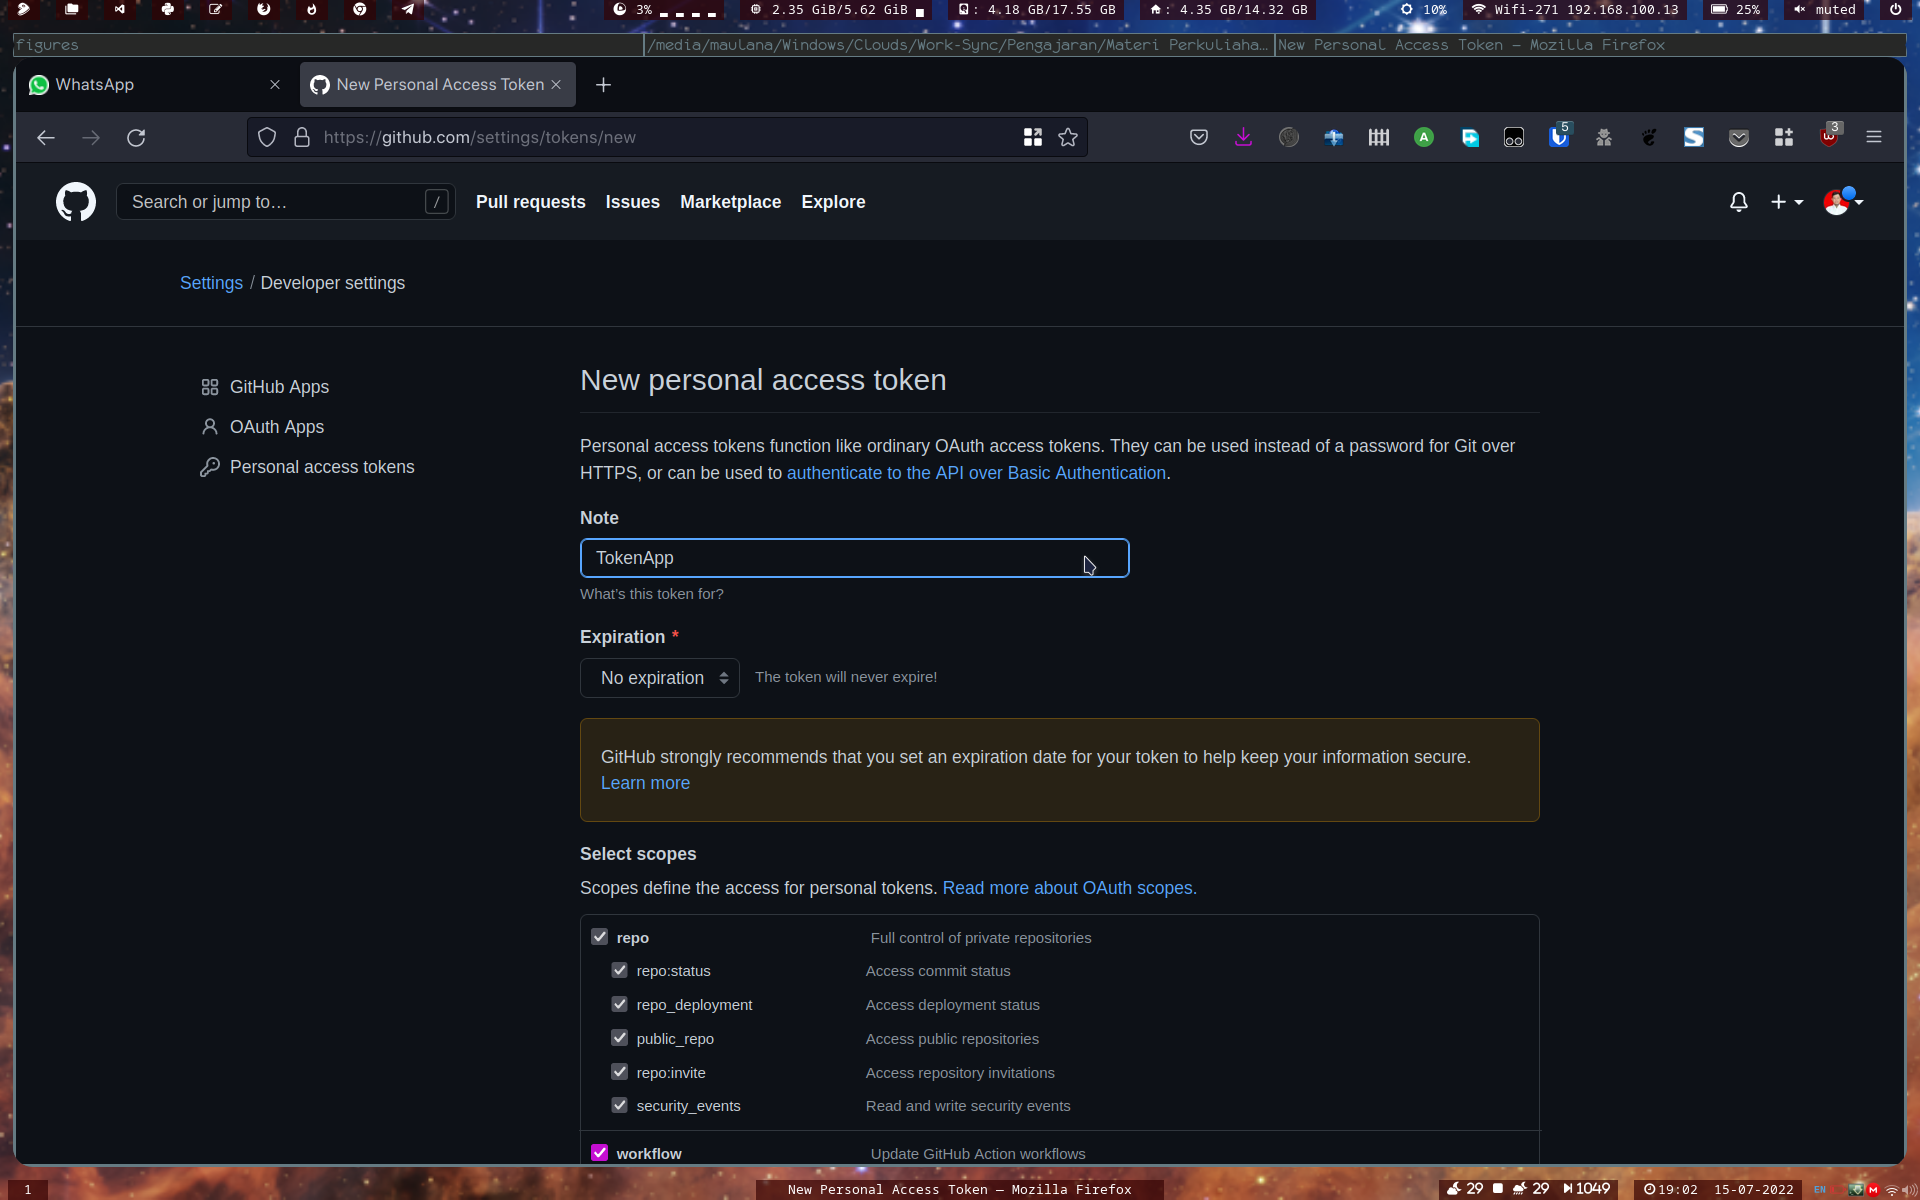
\includegraphics[width=0.8\textwidth]{figures/token4.png}
			\label{fig.token4}
		\end{figure}
		\item GitHub akan membuat kode unik yang harus disimpan dan tidak boleh dimasukkan ke folder git. Simpan baik baik. 
		\begin{figure}[H]
			\centering
			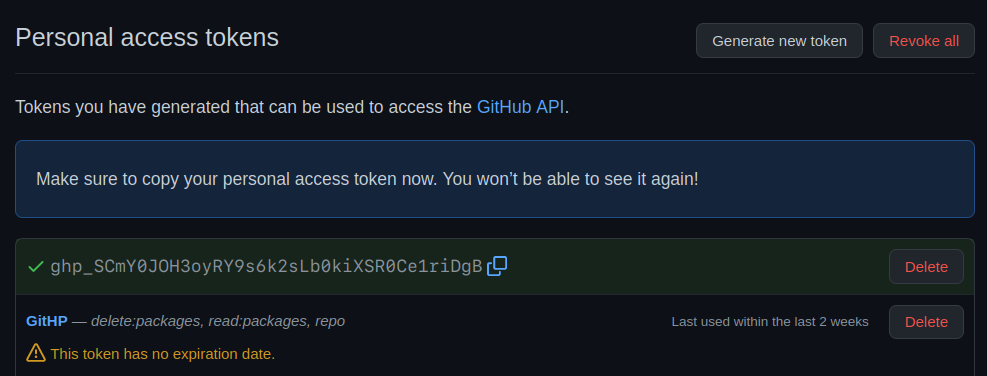
\includegraphics[width=0.8\textwidth]{figures/token5.png}
			\label{fig.token5}
		\end{figure}
		\item Kopi kode tersebut karena tidak akan muncul lagi.
	\end{enumerate}

  %%%%%%%%%%%%%%
  % Bab 3 %
  %%%%%%%%%%%%%%

\chapter{Praktikum 1}

	\section{Membuat Folder GIT}
	Di bagian ini mahasiswa diajarkan bagaimana melakukan pembuatan projek git, menambahkan file ke git, melakukan pelabelan, dan mengunggah ke repositori. Mahasiswa diwajibkan untuk menyelesaikan \textbf{Persiapan Praktikum} sebelum masuk ke tahapan ini.
	
	\section{Tutorial}
	\begin{enumerate}
		\item Buka \textbf{Git Bash} jika menggunakan \textbf{Windows} atau \textbf{Terminal} jika menggunakan \textbf{Linux}. Keduanya sama-sama memiliki antarmuka dan perintah yang sama.
		\begin{figure}[H]
			\centering
			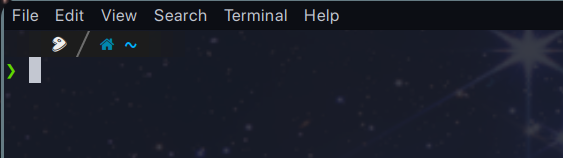
\includegraphics[width=0.8\textwidth]{figures/prak1-1.png}
		\end{figure}
		\item Sebelum masuk ke pembuatan projek, sebaiknya aplikasi \textbf{git} dikonfigurasikan terlebih dahulu dengan perintah berikut:
		\begin{verbatim}
			git config --global user.name "Your Name"
			git config --global user.email "youremail@yourdomain.com"
			(Keterangan : Mengeset Nama dan E-Mail dalam config)
		\end{verbatim}
		\item Kemudian cek dengan perintah:
		\begin{verbatim}
			git config --list
			(Keterangan : Melihat daftar konfigurasi)
		\end{verbatim}
		\item Konfigurasi ini dapat dilihat di folder \textbf{\%USERPROFILE\%/.gitconfig} (\textbf{Windows}) atau di \textbf{\$HOME/.gitconfig} (\textbf{Linux})
		\begin{figure}[H]
			\centering
			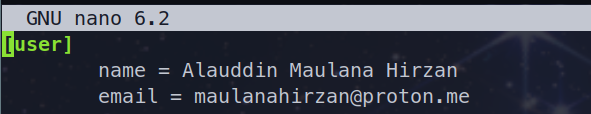
\includegraphics[width=0.8\textwidth]{figures/prak1-0.png}
		\end{figure}
		\item Buatlah sebuah folder dan masuk ke dalam folder tersebut dengan menggunakan perintah berikut:
		\begin{verbatim}
			mkdir PraktikumOSS
			cd PraktikumOSS
		\end{verbatim}
		\begin{figure}[H]
			\centering
			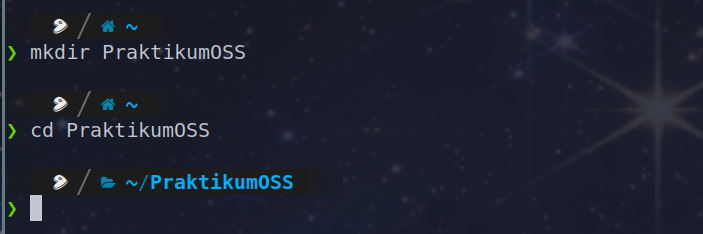
\includegraphics[width=0.8\textwidth]{figures/prak1-2.png}
		\end{figure}
	\item Buatlah \textbf{Sebuah File} dengan menggunakan \textbf{Notepad} atau \textbf{Editor Lain} dengan isi sebagai berikut, dan simpan sebagai \textbf{Praktikum1.txt} di dalam folder \textbf{PraktikumOSS}.
	\begin{verbatim}
		<Nama> : <NIM> : <Asal>
	\end{verbatim}
	\begin{figure}[H]
		\centering
		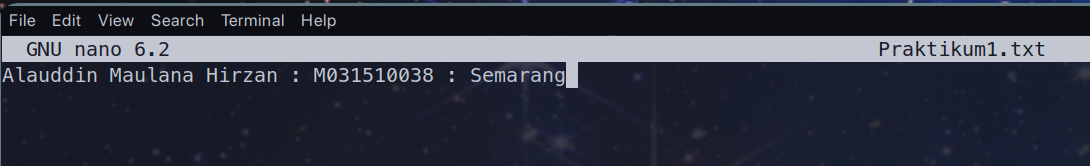
\includegraphics[width=0.8\textwidth]{figures/prak1-3.png}
	\end{figure}
	\item Setelah file tersimpan dengan baik, waktunya membuat projek di dalam folder tersebut. Gunakan perintah berikut untuk mengubah folder tersebut menjadi folder GIT:
	\begin{verbatim}
		git init
		(Keterangan : Mengubah Folder biasa menjadi Folder GIT)
	\end{verbatim}
	\begin{figure}[H]
		\centering
		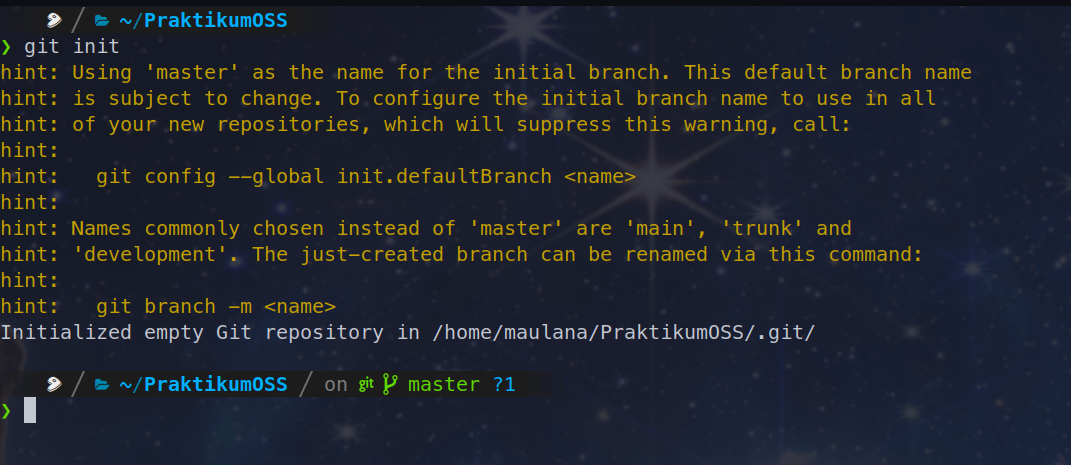
\includegraphics[width=0.8\textwidth]{figures/prak1-4.png}
	\end{figure}
	\item Folder ini sudah menjadi folder GIT, namun belum bisa mengunggah ke repositori. Untuk dapat mengunggah, gunakan perintah berikut:
	\begin{verbatim}
		git add -Av 
		(Keterangan : Tambahkan semua file dan tampilkan log)
	\end{verbatim}
	\begin{figure}[H]
		\centering
		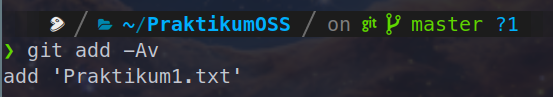
\includegraphics[width=0.8\textwidth]{figures/prak1-5.png}
	\end{figure}
	\item Berikutnya adalah memberikan label atas file-file yang ingin diunggah. Kita sebut ini sebagai \textbf{\textit{COMMIT}}. Gunakan perintah berikut untuk melabeli unggahan (bukan FILE):
	\begin{verbatim}
		git commit -m "Versi 0.0.1 - File Baru"
		(Keterangan : Membuat commit atau label untuk unggahan yang akan dilakukan)
	\end{verbatim}
	\begin{figure}[H]
		\centering
		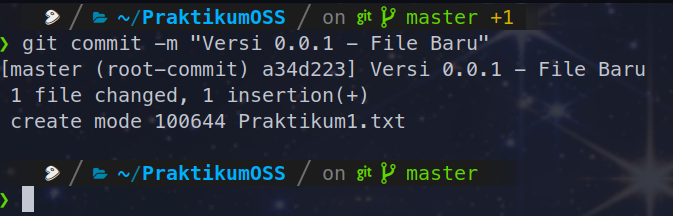
\includegraphics[width=0.8\textwidth]{figures/prak1-6.png}
	\end{figure}
	\item Namun untuk mengunggah folder ini, kita memutuhkan yang namanya \textbf{\textit{Repository}} (bukan akun) yang ada di dalam GitHub. Buka \url{github.com} dan buatlah Repositori baru dengan meng-klik \textbf{New}
	\begin{figure}[H]
		\centering
		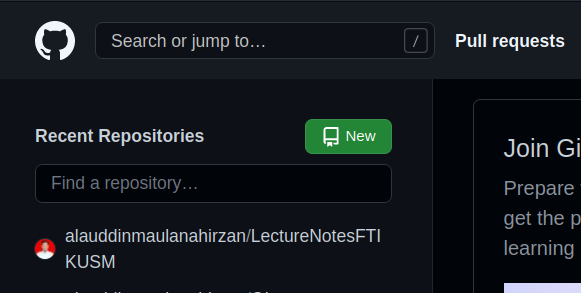
\includegraphics[width=0.8\textwidth]{figures/prak1-7.png}
	\end{figure}
	\item Beri nama Repositori dengan \textbf{PraktikumOSS-[4 DIGIT NIM Terakhir]}. Untuk membedakan mahasiswa satu dengan yang lainnya.
	\begin{figure}[H]
		\centering
		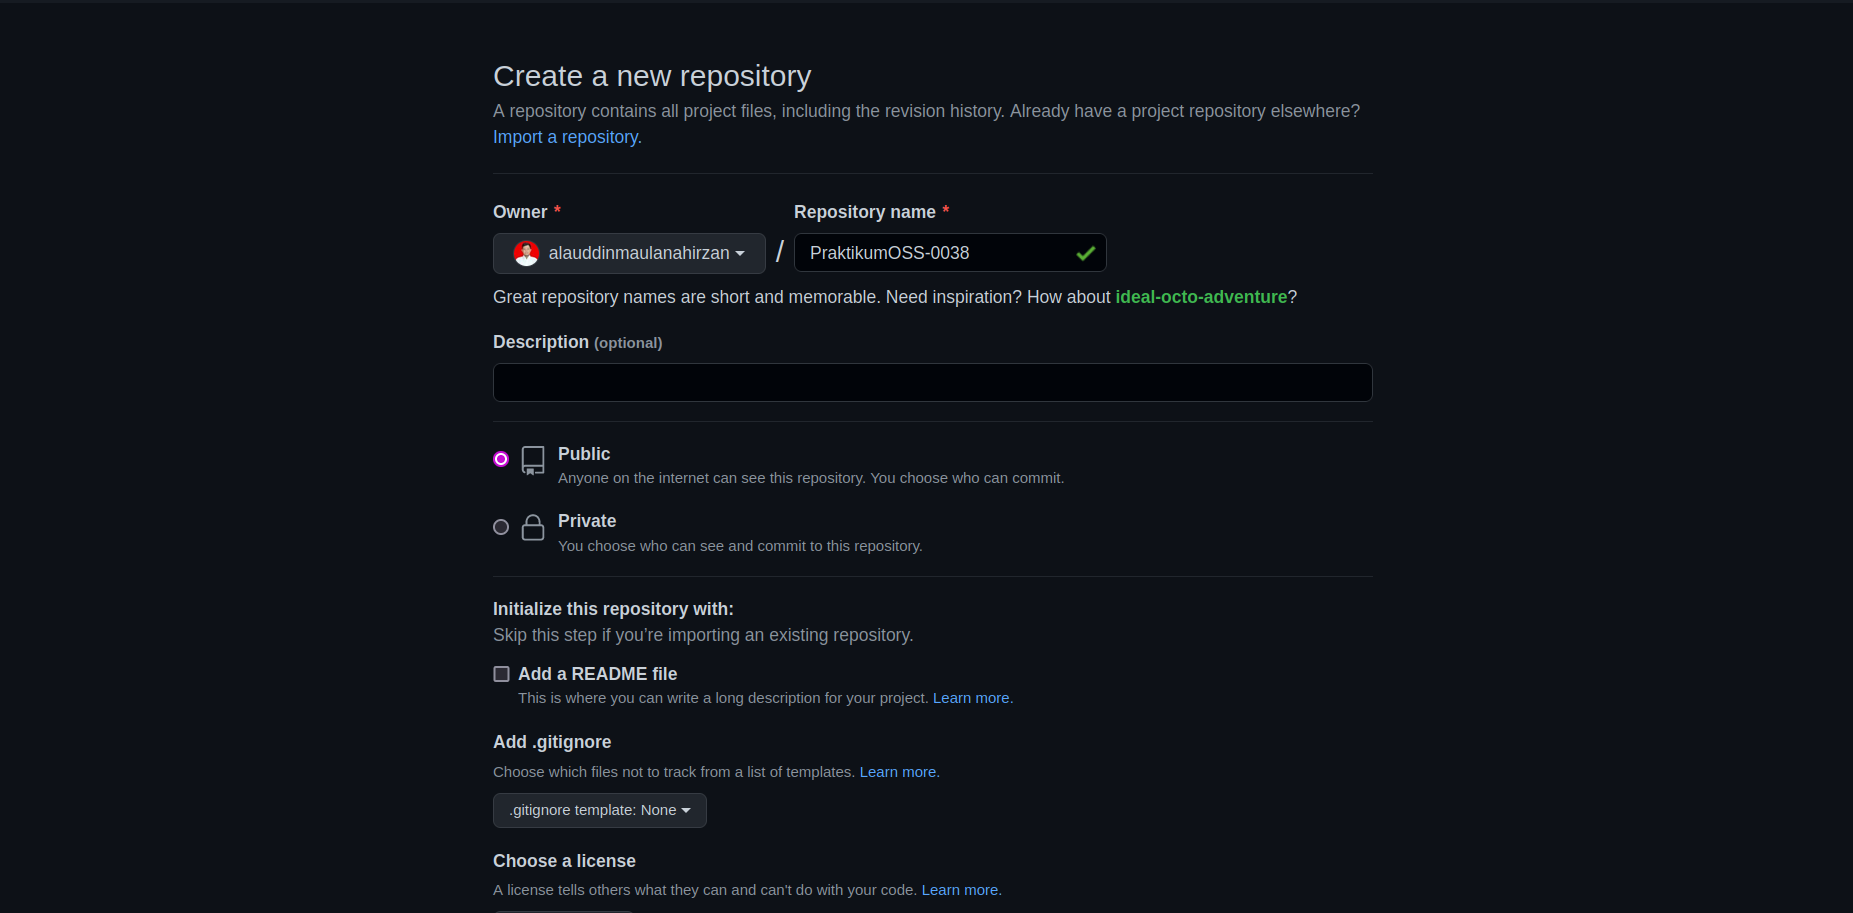
\includegraphics[width=0.8\textwidth]{figures/prak1-8.png}
	\end{figure}
	\item Kemudian klik \textbf{Create Repository} yang ada di bagian bawah.
	\item Berikutnya kita akan diarahkan ke halaman repositori tersebut. Lalu \textbf{Kopi} alamat yang ada di sana.
	\begin{figure}[H]
		\centering
		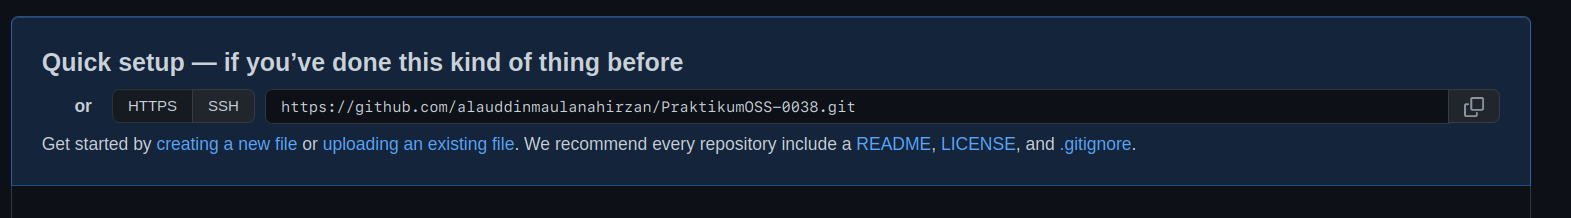
\includegraphics[width=0.8\textwidth]{figures/prak1-9.png}
	\end{figure}
	Kembali ke \textbf{Git Bash} atau terminal dan masukkan perintah berikut:
	\begin{verbatim}
		git remote add origin [alamat dari langkah sebelumnya]
		(Keterangan : Mengeset [alamat] sebagai tujuan unggahan)
	\end{verbatim}
	\begin{figure}[H]
		\centering
		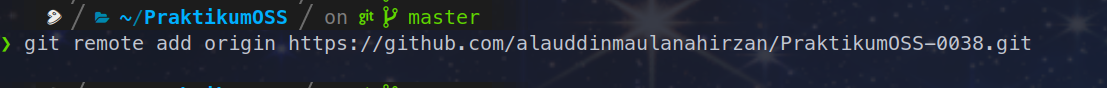
\includegraphics[width=0.8\textwidth]{figures/prak1-10.png}
	\end{figure}
	\item Sebelum melakukan penggunggahan, sebaiknya mengkonfigurasikan GIT agar menyimpan \textit{credentials} sehingga tidak perlu lagi memasukkan token ketika login. Masukkan perintah berikut:
	\begin{verbatim}
		git config --global credential.helper store
		(Keterangan : Menyimpan username dan token ketika mengunggah)
	\end{verbatim}
	\begin{figure}[H]
		\centering
		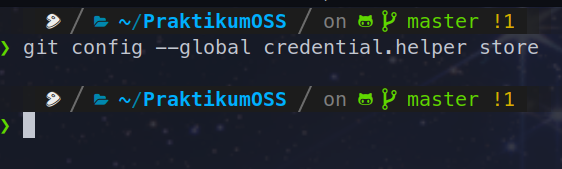
\includegraphics[width=0.8\textwidth]{figures/prak1-14.png}
	\end{figure}
	\item Kini GIT siap melakukan pengunggahan. Karena masih pertama kali gunakan perintah berikut: (Catatan: \textbf{PASSWORD diisi dengan TOKEN, dan INPUT TIDAK AKAN TERLIHAT})
	\begin{verbatim}
		git push --set-upstream origin main -f 
		(Keterangan : Perintah ini akan mengeset origin sebagai tujuan dan 
		-f akan memaksa unggahan)
	\end{verbatim}
	\begin{figure}[H]
		\centering
		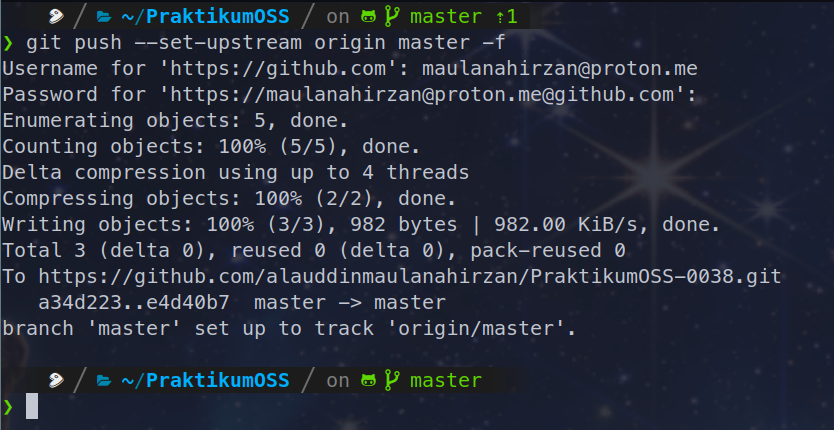
\includegraphics[width=0.8\textwidth]{figures/prak1-15.png}
	\end{figure}
	\item Folder sudah terunggah, buka repositori tadi untuk melihat hasilnya.
	\begin{figure}[H]
		\centering
		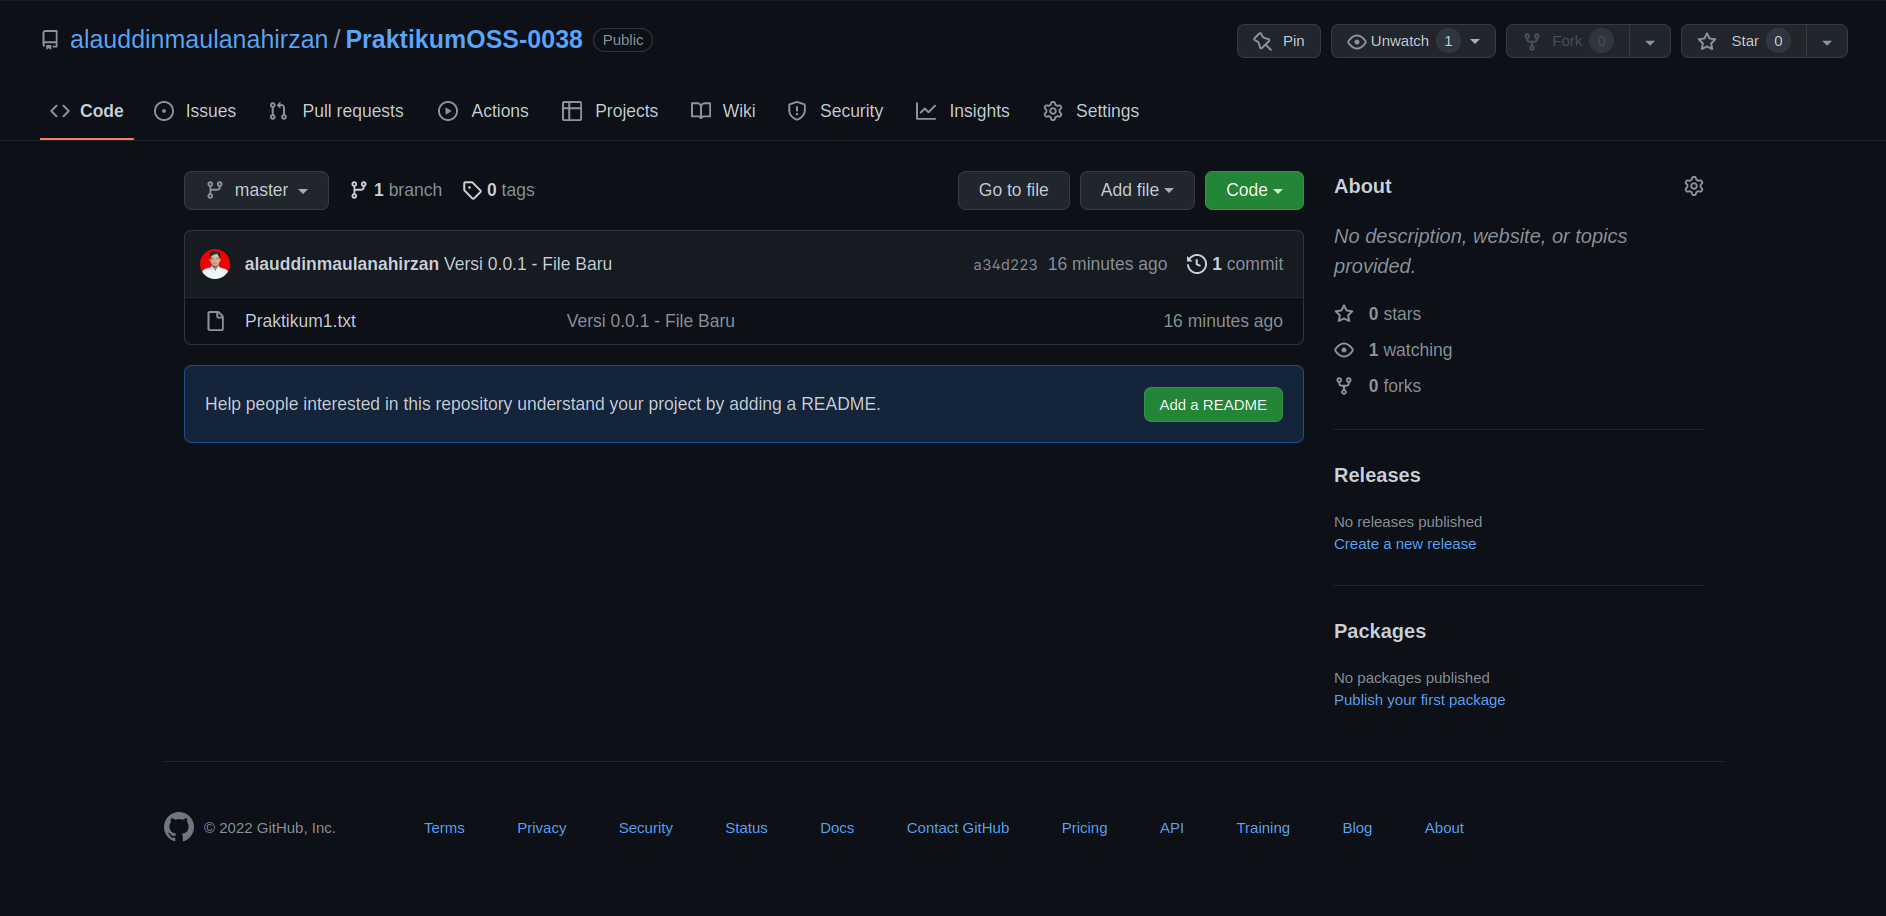
\includegraphics[width=0.8\textwidth]{figures/prak1-12.png}
	\end{figure}
	\item Dan jika dibuka berisi
	\begin{figure}[H]
		\centering
		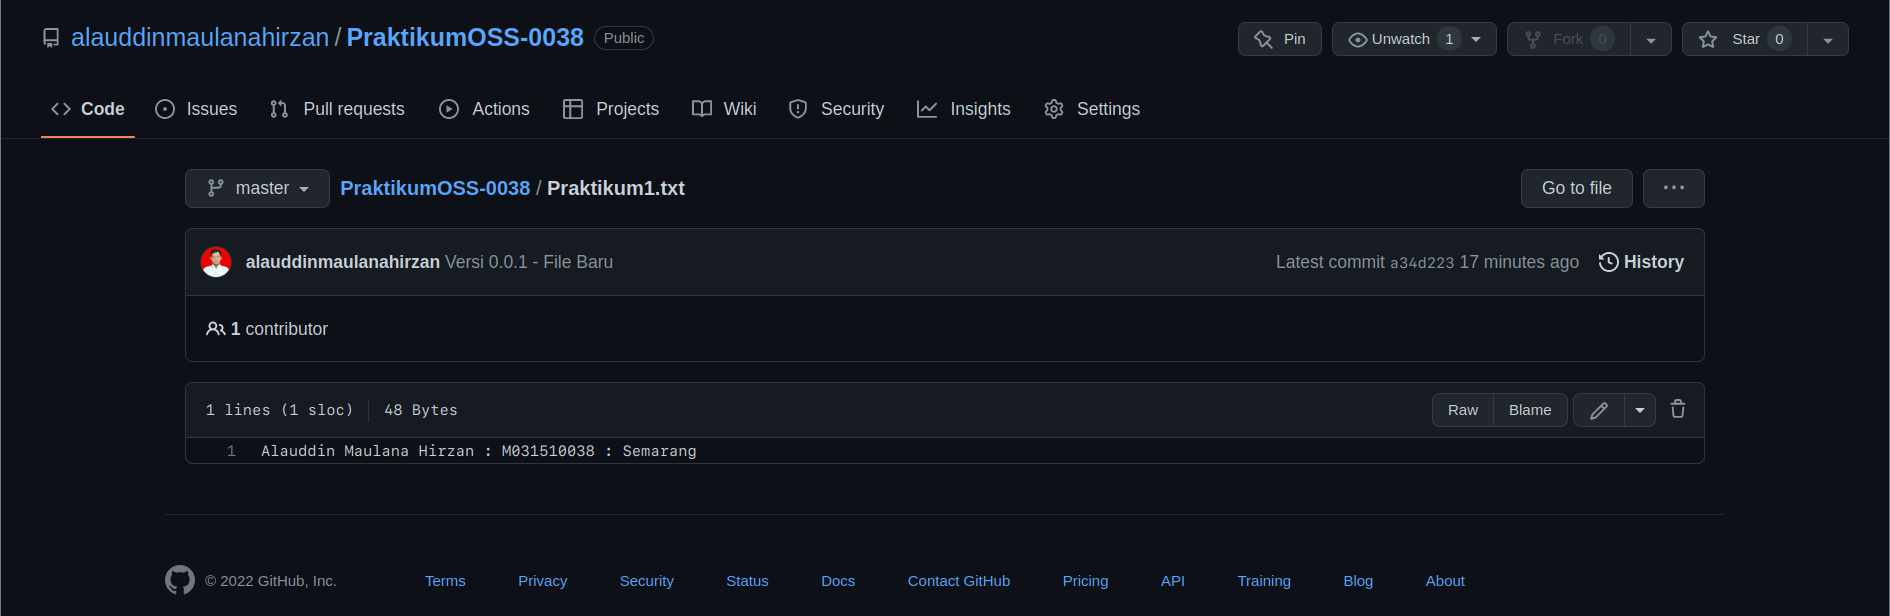
\includegraphics[width=0.8\textwidth]{figures/prak1-13.png}
	\end{figure}
	\item Kumpulkan hasil yang sudah dibuat ke e-Learning yang sudah disediakan
	\item Praktikum 1 Selesai
	\end{enumerate}

  %%%%%%%%%%%%%%
  % Bab 4 %
  %%%%%%%%%%%%%%

\chapter{Praktikum 2}
	\section{Kloning dan Update Repositori}
	Di bagian ini mahasiswa diajarkan bagaimana melakukan kloning repositori yang sudah dibuat sebelumnya, kemudian melakukan perubahan yang ada di dalam file, dan mengunggahnya kembali ke repositori. Mahasiswa diwajibkan untuk menyelesaikan \textbf{Praktikum 1} sebelum masuk ke tahapan ini.
	
	\section{Tutorial}
	\begin{enumerate}
		\item Buka \textbf{Git Bash} atau \textbf{Terminal}
		\item Hapus folder \textbf{PraktikumOSS-[NIM]]}
		\begin{itemize}
			\item Hapus folder \textbf{PraktikumOSS} menggunakan \textbf{File Explorer} jika menggunakan Windows
			\item Jika penghapusan dilakukan secara manual melalui perintah seperti berikut:
			\begin{verbatim}
				cd .. (Keterangan : Naik Satu Folder)
				rm -rf PraktikumOSS (Jika Linux) / rmdir PraktikumOSS (Jika Windows)
			\end{verbatim}
		\end{itemize}
		\item Di tempat saat ini (\textbf{Bukan PraktikumOSS-[NIM]}), masukkan perintah berikut untuk melakukan kloning repositori:
		\begin{verbatim}
			git clone [url repository]
			(Keterangan : Melakukan kloning dari url repository ke dalam folder)
		\end{verbatim}
		\begin{figure}[H]
			\centering
			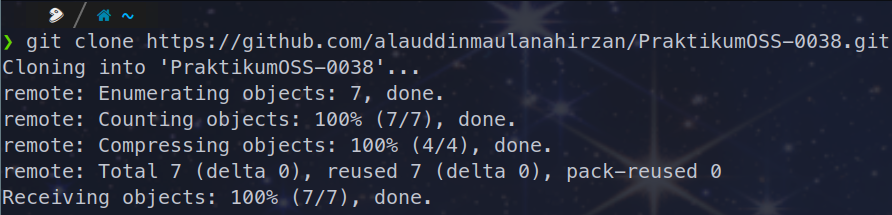
\includegraphics[width=0.8\textwidth]{figures/prak2-1.png}
		\end{figure}
		\item Kemudian masuk ke folder yang sudah di klon dengan perintah berikut:
		\begin{verbatim}
			cd PraktikumOSS-[4 Digit NIM]
		\end{verbatim}
		\begin{figure}[H]
			\centering
			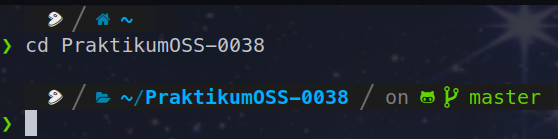
\includegraphics[width=0.8\textwidth]{figures/prak2-2.png}
		\end{figure}
		\item Buka file \textbf{Praktikum1.txt} dengan menggunakan Notepad maupun Editor Lainnya. Dan masukkan data sebagai berikut tepat di bawah data yang sudah ada
		\begin{verbatim}
			Mata Kuliah : Open Source System
			Catatan : Praktikum dengan menggunakan GIT
		\end{verbatim}
		\begin{figure}[H]
			\centering
			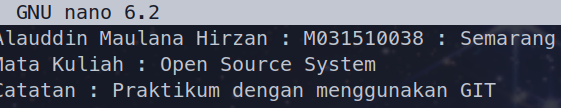
\includegraphics[width=0.8\textwidth]{figures/prak2-3.png}
		\end{figure}
		\item Data perubahan ini akan terdeteksi oleh GIT. Gunakan perintah:
		\begin{verbatim}
			git add -Av
		\end{verbatim}
		\begin{figure}[H]
			\centering
			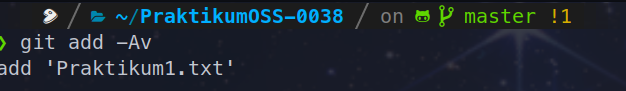
\includegraphics[width=0.8\textwidth]{figures/prak2-4.png}
		\end{figure}
		\item setelah itu lakukan \textit{Commit} dengan perintah berikut:
		\begin{verbatim}
			git commit -m "Versi 0.0.2 - File Update"
		\end{verbatim}
		\item Lalu unggah dengan perintah 
		\begin{verbatim}
			git push
		\end{verbatim}
		\item Cek file yang telah dirubah yang ada di dalam repositori
		\begin{figure}[H]
			\centering
			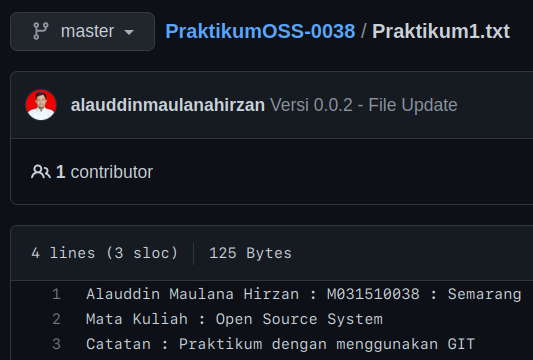
\includegraphics[width=0.8\textwidth]{figures/prak2-5.png}
		\end{figure}
	\item Praktikum 2 Selesai
	\end{enumerate}

  	\section{Tugas Mandiri}
  		Mahasiswa diwajibkan mengerjakan sesi mandiri ini setelah mengerjakan bagian \textbf{Tutorial}
  		\begin{enumerate}
  			\item Buatlah satu file dengan nama \textbf{README.md} di folder \textbf{PraktikumOSS-[NIM]}
  			\item Dengan menggunakan \textbf{Notepad} atau \textbf{Editor Lain}, masukkan data berikut:
  				\begin{verbatim}
  					# Praktikum Open Source System
  					#### Ditulis oleh : <NIM> <Nama>
  					#### Semester : <Semester>
  					#### Tanggal Praktikum : <Tanggal>
  
  					Repositori ini merupakan hasil praktikum *Open Source System* yang nantinya 
  					dapat digunakan untuk menyimpan semua koding-koding yang dibuat.
  				\end{verbatim}
  			\item \textbf{Tambahkan}, \textbf{Commit} dengan pesan "Tugas Mandiri 1", dan \textbf{Push} ke Repositori
  			\item Hasil akhir harus seperti berikut:
  				\begin{figure}[H]
  					\centering
  					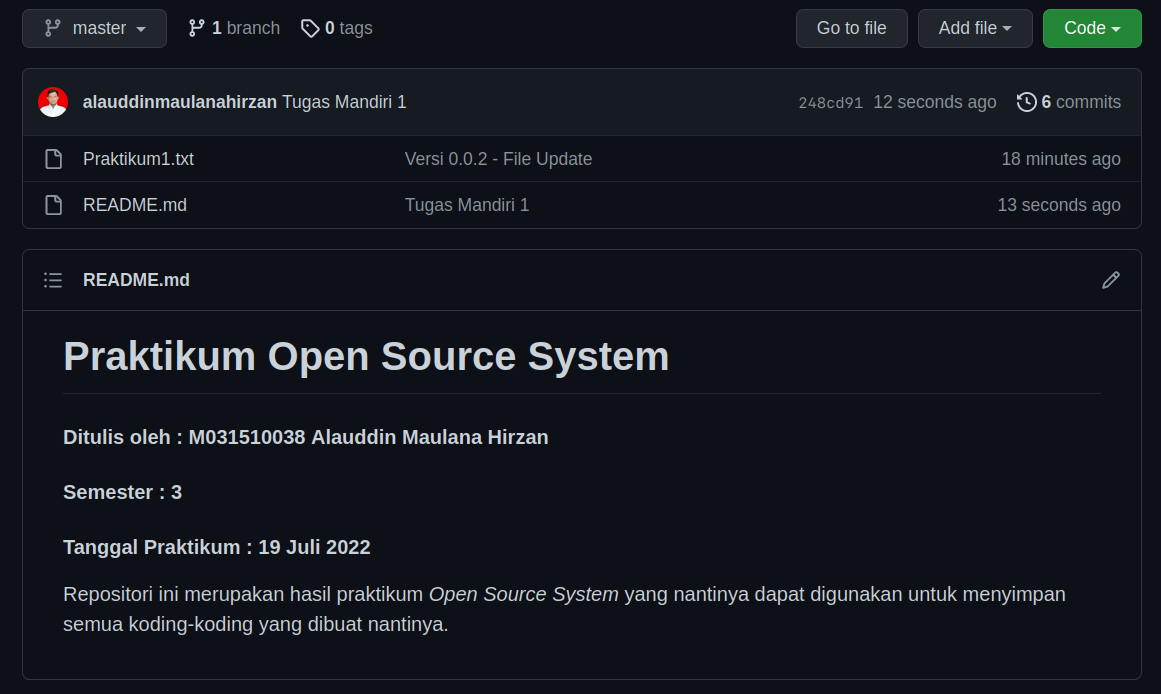
\includegraphics[width=0.73\textwidth]{figures/prak2-6.png}
  				\end{figure}
  			\item Kumpulkan hasil yang sudah dibuat ke e-Learning yang sudah disediakan
  		\end{enumerate}
  	
  	 %%%%%%%%%%%%%%
  	% Bab 5 %
  	%%%%%%%%%%%%%%
  	
  	\chapter{Praktikum 3}
  		\section{Percabangan Repositori}
  	Di bagian ini mahasiswa diajarkan bagaimana membuat percabangan (branch) dari repositori utama yang sudah dibuat sebelumnya, kemudian melakukan perubahan yang ada di dalam file, dan mengunggahnya kembali ke repositori sebagai cabang yang berbeda. Mahasiswa diwajibkan untuk menyelesaikan \textbf{Praktikum 2} sebelum masuk ke tahapan ini.
  	
  	\section{Tutorial}
  	\begin{enumerate}
  		\item Buka folder sebelumnya (\textbf{PraktikumOSS-[NIM]}) dengan menggunakan \textbf{Git Bash} atau \textbf{Terminal}
  		\item Pastikan posisi \textbf{Git Bash} atau \textbf{Terminal} sudah berada di folder tersebut
  		\begin{figure}[H]
  			\centering
  			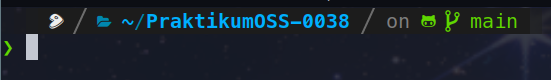
\includegraphics[width=0.73\textwidth]{figures/prak3-1.png}
  		\end{figure}
  		\item Untuk memulai cabang baru dari repositori lokal saat ini, gunakan perintah berikut:
  		\begin{itemize}
  			\item Perintah Alternatif 1
  			\begin{verbatim}
  				git branch Cabang1
  				(Keterangan : Buat cabang baru dengan nama Cabang1)
  				git checkout Cabang1
  				(Keterangan : Pindah cabang aktif ke Cabang1)
  			\end{verbatim}
  			\begin{figure}[H]
  				\centering
  				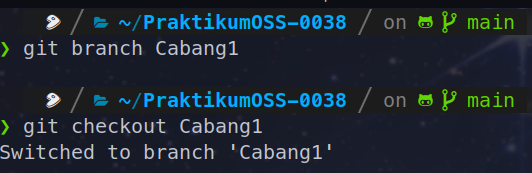
\includegraphics[width=0.73\textwidth]{figures/prak3-2.png}
  			\end{figure}
  			\item Perintah Alternatif 2
  			\begin{verbatim}
  				git checkout -b Cabang1
  				(Keterangan : Buat dan pindah cabang aktif ke Cabang1)
  			\end{verbatim}
  			\begin{figure}[H]
  				\centering
  				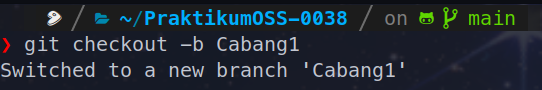
\includegraphics[width=0.73\textwidth]{figures/prak3-3.png}
  			\end{figure}
  		\end{itemize}
  		\item Sesudah itu, cabang akan dialihkan ke \textbf{Cabang1}, bukan \textbf{main} lagi. Kita dapat memodifikasi sesuka kita di cabang ini tanpa harus mengganggu cabang utama.
  		\item Dengan menggunakan \textbf{Notepad} atau \textbf{Editor Lainnya}, buatlah sebuah file dengan nama \textbf{File Cabang Baru.txt}.
  		\item Kemudian isi file tersebut dengan isi sebagai berikut:
  		\begin{verbatim}
  			File ini merupakan file yang hanya bisa dilihat di Cabang1. Sehingga tidak 
  			akan muncul di Cabang Utama (Main)
  		\end{verbatim}
  	\begin{figure}[H]
  		\centering
  		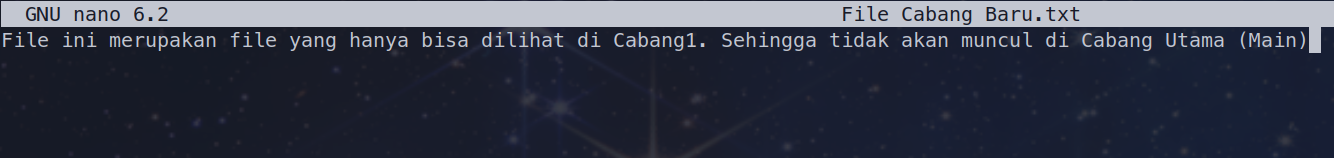
\includegraphics[width=0.73\textwidth]{figures/prak3-4.png}
  	\end{figure}
  	\item Masukkan file ke dalam \textbf{stage} dengan perintah
  	\begin{verbatim}
  		git add -Av
  	\end{verbatim}
  	\item Beri \textbf{Commit} baru ke cabang yang akan diunggah
  	\begin{verbatim}
  		git commit -m "File Cabang Baru"
  	\end{verbatim}
  	\item Lalu unggah dengan perintah berikut
  	\begin{verbatim}
  		git push --set-upstream origin Cabang1 -f
  		(Keterangan : Unggah Repositori ke Cabang1)
  	\end{verbatim}
  	\begin{figure}[H]
  	\centering
  	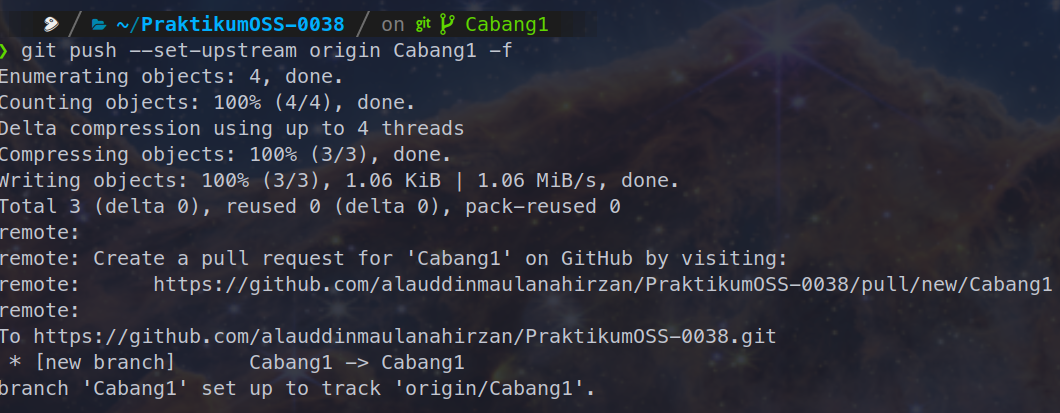
\includegraphics[width=0.73\textwidth]{figures/prak3-5.png}
  \end{figure}
	\item Cek apakah sudah terunggah sempurna di Repositori Remote
	\begin{figure}[H]
		\centering
		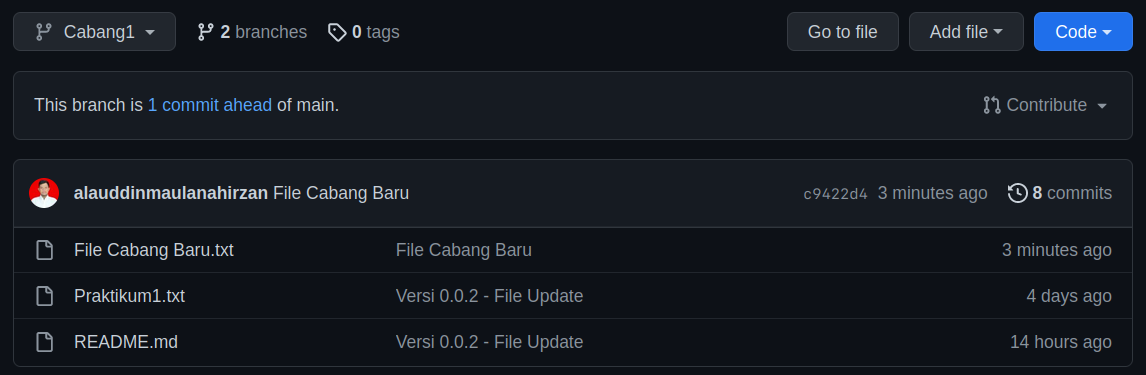
\includegraphics[width=0.73\textwidth]{figures/prak3-6.png}
	\end{figure}
	\item Jika berhasil maka \textbf{Cabang1} akan muncul di daftar Branch termasuk \textbf{File Baru} yang kita buat.
	\item Praktikum 3 Selesai
  	\end{enumerate}
  
  	\section{Tugas Mandiri}
  	\begin{enumerate}
  		\item Buat cabang baru dengan nama \textbf{Cabang2}
  		\item Buatlah file baru dengan nama \textbf{FIleCabang2.txt}
  		\item Isi dengan teks berikut:
  		\begin{verbatim}
  			File Tugas Mandiri Cabang 2
  		\end{verbatim}
  		\item Unggah ke Repositori Remote
  		\item Hasil screenshot mirip \textbf{Langkah 10}, kirimkan ke e-Learning
  	\end{enumerate}
  	
  	
  	
  	
  	
\end{document}
